\documentclass{standalone}
\usepackage{tikz}
\usepackage{amsmath}
\usepackage{xcolor}

\begin{document}

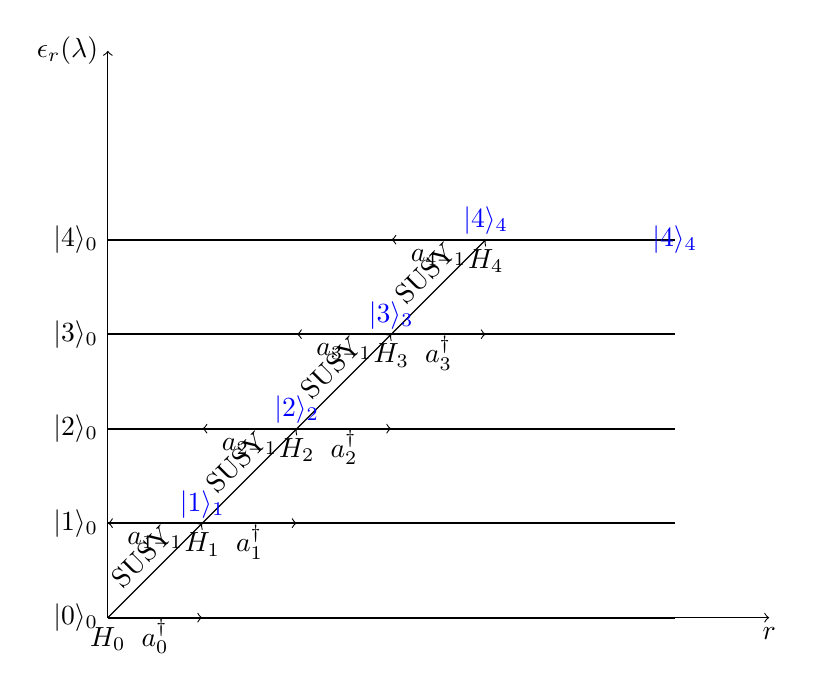
\begin{tikzpicture}[scale=1.2]

% Axes
\draw[->] (0,0) -- (7,0) node[below] {$r$};
\draw[->] (0,0) -- (0,6) node[left] {$\epsilon_r(\lambda)$};

% Horizontal lines and labels
\foreach \y/\label in {0/0, 1/1, 2/2, 3/3, 4/4} {
    \draw[thick] (0,\y) -- (6,\y);
    \node[left] at (0,\y) {$|\y\rangle_0$};
}

% Vertical Hamiltonians
\node[below] at (0,0) {$H_0$};
\node[below] at (1,1) {$H_1$};
\node[below] at (2,2) {$H_2$};
\node[below] at (3,3) {$H_3$};
\node[below] at (4,4) {$H_4$};

% Diagonal SUSY arrows
\foreach \i in {0,1,2,3} {
    \draw[->] (\i,\i) -- (\i+1,\i+1) node[midway, sloped, above] {SUSY};
}

% Operators and states
\foreach \i/\j in {0/1, 1/2, 2/3, 3/4} {
    \draw[->] (\i,\i) -- (\i+1,\i);
    \node at (\i+0.5,\i-0.2) {$a_{\i}^\dagger$};
}

\foreach \i/\j in {1/0, 2/1, 3/2, 4/3} {
    \draw[->] (\i,\i) -- (\i-1,\i);
    \node at (\i-0.5,\i-0.2) {$a_{\i-1}$};
}

% Blue labels
\node[blue] at (1,1.2) {$|1\rangle_1$};
\node[blue] at (2,2.2) {$|2\rangle_2$};
\node[blue] at (3,3.2) {$|3\rangle_3$};
\node[blue] at (4,4.2) {$|4\rangle_4$};

% Edge state
\node[blue] at (6,4) {$|4\rangle_4$};

\end{tikzpicture}

\end{document}